\chapter{Memory and Performance Optimization}

\section{Introduction}

Modern software performance is heavily influenced by memory behavior. While CPU frequencies have increased over the years, memory latency improvements have been much slower. As a result, understanding operating system memory concepts is essential for building scalable, high-performance systems.

In system design interviews and real-world engineering, memory efficiency often determines:

\begin{itemize}
\item Application throughput
\item Response latency
\item Scalability
\item Resource utilization
\item Infrastructure cost
\end{itemize}

This chapter connects operating system memory management concepts with practical software engineering performance optimization.

%====================================================
\section{Performance Fundamentals}
%====================================================

\subsection{Definition}

Performance measures how efficiently a system completes work.

Common metrics include:

\begin{itemize}
\item Throughput
\item Latency
\item CPU Utilization
\item Memory Usage
\item Requests Per Second (RPS)
\item Tail Latency (P95, P99)
\end{itemize}

\subsection{Performance Equation}

\[
Performance = \frac{Work}{Time}
\]

\subsection{Key Observation}

Many applications are not CPU-bound but memory-bound.

%====================================================
\section{CPU Cache Hierarchy}
%====================================================

\subsection{Motivation}

Main memory is much slower than CPU execution speed.

Caches reduce memory access latency.

\subsection{Hierarchy}

\begin{figure}[h]
\centering
\begin{tikzpicture}

\node[draw] (cpu) {CPU Registers};

\node[draw,below=0.8cm of cpu] (l1) {L1 Cache};

\node[draw,below=0.8cm of l1] (l2) {L2 Cache};

\node[draw,below=0.8cm of l2] (l3) {L3 Cache};

\node[draw,below=0.8cm of l3] (ram) {Main Memory};

\node[draw,below=0.8cm of ram] (disk) {Storage};

\draw[->] (cpu)--(l1);
\draw[->] (l1)--(l2);
\draw[->] (l2)--(l3);
\draw[->] (l3)--(ram);
\draw[->] (ram)--(disk);

\end{tikzpicture}
\caption{Memory Hierarchy}
\end{figure}

\subsection{Characteristics}

\begin{table}[h]
\centering
\begin{tabular}{|c|c|c|}
\hline
Level & Speed & Size \\
\hline
Registers & Fastest & Smallest \\
L1 Cache & Very Fast & Small \\
L2 Cache & Fast & Medium \\
L3 Cache & Slower & Larger \\
RAM & Slow & Large \\
Disk & Slowest & Huge \\
\hline
\end{tabular}
\caption{Memory Hierarchy Characteristics}
\end{table}

%====================================================
\section{Cache Locality}
%====================================================

\subsection{Definition}

Cache locality refers to the tendency of programs to access the same or nearby memory locations repeatedly.

\subsection{Importance}

Good locality improves:

\begin{itemize}
\item Cache hit rate
\item CPU efficiency
\item Throughput
\end{itemize}

Poor locality causes:

\begin{itemize}
\item Cache misses
\item Memory stalls
\item Increased latency
\end{itemize}

%====================================================
\section{Spatial Locality}
%====================================================

\subsection{Definition}

If a memory location is accessed, nearby locations are likely to be accessed soon.

\subsection{Example}

\begin{verbatim}
for(int i=0;i<n;i++)
    sum += arr[i];
\end{verbatim}

Sequential array access exhibits strong spatial locality.

\subsection{Benefit}

Entire cache lines become useful.

%====================================================
\section{Temporal Locality}
%====================================================

\subsection{Definition}

Recently accessed memory is likely to be accessed again soon.

\subsection{Example}

\begin{verbatim}
count++;
count++;
count++;
\end{verbatim}

The variable remains in cache.

\subsection{Benefit}

Reduces repeated memory fetches.

%====================================================
\section{Cache Lines}
%====================================================

\subsection{Definition}

Caches transfer data in fixed-size units called cache lines.

Typical size:

\[
64 \text{ Bytes}
\]

\subsection{Illustration}

\begin{figure}[h]
\centering

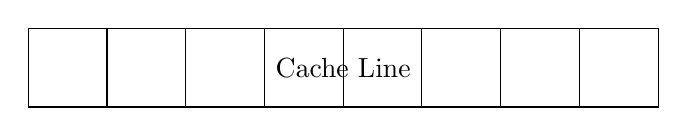
\begin{tikzpicture}

\draw (0,0) rectangle (8,1);

\foreach \x in {1,2,3,4,5,6,7}
{
\draw (\x,0)--(\x,1);
}

\node at (4,0.5) {Cache Line};

\end{tikzpicture}

\caption{Cache Line}
\end{figure}

\subsection{Interview Insight}

Most cache optimization discussions revolve around cache lines.

%====================================================
\section{False Sharing}
%====================================================

\subsection{Definition}

False sharing occurs when multiple threads update different variables located on the same cache line.

\subsection{Example}

\begin{verbatim}
Thread A -> counter1
Thread B -> counter2
\end{verbatim}

Even though variables differ, cache invalidations occur.

\subsection{Effects}

\begin{itemize}
\item Cache contention
\item Reduced scalability
\item Throughput degradation
\end{itemize}

\subsection{Solution}

Padding structures to separate cache lines.

%====================================================
\section{TLB Overview}
%====================================================

\subsection{Definition}

TLB stands for Translation Lookaside Buffer.

It caches virtual-to-physical address translations.

\subsection{Address Translation}

\[
Virtual Address
\rightarrow
TLB
\rightarrow
Physical Address
\]

\subsection{Purpose}

Avoid expensive page table lookups.

%====================================================
\section{TLB Performance Impact}
%====================================================

\subsection{TLB Hit}

Address translation is immediate.

\subsection{TLB Miss}

Page table lookup is required.

\subsection{Impact}

TLB misses can significantly increase memory access time.

\subsection{Interview Insight}

Many high-performance systems use huge pages to reduce TLB misses.

%====================================================
\section{Memory Access Costs}
%====================================================

Approximate latencies:

\begin{table}[h]
\centering
\begin{tabular}{|c|c|}
\hline
Operation & Latency \\
\hline
Register Access & 1 Cycle \\
L1 Cache & 4 Cycles \\
L2 Cache & 12 Cycles \\
L3 Cache & 40 Cycles \\
RAM Access & 100-300 Cycles \\
SSD Access & Thousands of Cycles \\
\hline
\end{tabular}
\caption{Memory Access Costs}
\end{table}

\subsection{Observation}

A RAM access can be hundreds of times slower than an L1 cache access.

%====================================================
\section{Branch Prediction}
%====================================================

\subsection{Definition}

Modern CPUs predict branch outcomes.

\subsection{Example}

\begin{verbatim}
if(x > 0)
    doWork();
\end{verbatim}

CPU predicts likely path.

\subsection{Correct Prediction}

Pipeline continues smoothly.

\subsection{Misprediction}

Pipeline flush occurs.

\subsection{Impact}

Can significantly affect performance.

%====================================================
\section{Pipeline Effects}
%====================================================

\subsection{Pipeline}

CPU instructions execute in stages.

\subsection{Benefits}

\begin{itemize}
\item Higher throughput
\item Better CPU utilization
\end{itemize}

\subsection{Problems}

\begin{itemize}
\item Branch mispredictions
\item Cache misses
\item Data hazards
\end{itemize}

\subsection{Result}

Pipeline stalls reduce performance.

%====================================================
\section{Memory Allocation Costs}
%====================================================

\subsection{Dynamic Allocation}

Examples:

\begin{verbatim}
malloc()
new
\end{verbatim}

\subsection{Costs}

\begin{itemize}
\item Metadata management
\item Synchronization
\item Fragmentation
\item Cache disruption
\end{itemize}

\subsection{Optimization}

Use:

\begin{itemize}
\item Memory pools
\item Object pools
\item Arena allocators
\end{itemize}

%====================================================
\section{NUMA Effects}
%====================================================

\subsection{NUMA}

Non-Uniform Memory Access.

\subsection{Concept}

Memory near a CPU is faster than remote memory.

\begin{figure}[h]
\centering
\begin{tikzpicture}

\node[draw] (cpu1) {CPU 1};
\node[draw,right=5cm of cpu1] (cpu2) {CPU 2};

\node[draw,below=1cm of cpu1] (mem1) {Memory 1};
\node[draw,below=1cm of cpu2] (mem2) {Memory 2};

\draw (cpu1)--(mem1);
\draw (cpu2)--(mem2);

\draw[dashed] (cpu1)--(mem2);
\draw[dashed] (cpu2)--(mem1);

\end{tikzpicture}
\caption{NUMA Architecture}
\end{figure}

\subsection{Performance Implications}

Remote memory accesses are slower.

\subsection{Optimization}

Keep threads close to their memory.

%====================================================
\section{Memory Leaks}
%====================================================

\subsection{Definition}

Allocated memory that is never released.

\subsection{Example}

\begin{verbatim}
int* p = new int[100];
// Missing delete[]
\end{verbatim}

\subsection{Effects}

\begin{itemize}
\item Increased memory usage
\item Performance degradation
\item Application crashes
\end{itemize}

%====================================================
\section{Fragmentation}
%====================================================

\subsection{Internal Fragmentation}

Unused space inside allocated blocks.

\subsection{External Fragmentation}

Free memory exists but is scattered.

\subsection{Effects}

\begin{itemize}
\item Allocation failures
\item Increased memory overhead
\end{itemize}

%====================================================
\section{Garbage Collection Overview}
%====================================================

\subsection{Definition}

Automatic memory reclamation.

\subsection{Languages}

\begin{itemize}
\item Java
\item C\#
\item Go
\item Python
\end{itemize}

\subsection{Advantages}

\begin{itemize}
\item Simpler memory management
\item Reduced memory leaks
\end{itemize}

\subsection{Disadvantages}

\begin{itemize}
\item Pause times
\item CPU overhead
\item Memory overhead
\end{itemize}

%====================================================
\section{Performance Profiling}
%====================================================

\subsection{Definition}

Measuring where execution time is spent.

\subsection{Popular Tools}

Linux:

\begin{itemize}
\item perf
\item valgrind
\item gprof
\item flame graphs
\end{itemize}

Java:

\begin{itemize}
\item VisualVM
\item JProfiler
\item YourKit
\end{itemize}

\subsection{Goal}

Find bottlenecks before optimizing.

%====================================================
\section{Benchmarking Fundamentals}
%====================================================

\subsection{Definition}

Controlled measurement of performance.

\subsection{Rules}

\begin{itemize}
\item Warm up application
\item Measure multiple runs
\item Remove noise
\item Use realistic workloads
\end{itemize}

\subsection{Example}

\begin{verbatim}
Time taken:
Array Access = 10 ms

Linked List Access = 150 ms
\end{verbatim}

%====================================================
\section{Performance Case Study}
%====================================================

\subsection{Scenario}

Backend service processes millions of requests.

Initial implementation:

\begin{itemize}
\item Linked Lists
\item Frequent allocations
\item Poor cache locality
\end{itemize}

Problems:

\begin{itemize}
\item High latency
\item Low throughput
\end{itemize}

Optimization:

\begin{itemize}
\item Arrays
\item Object pooling
\item Reduced allocations
\end{itemize}

Result:

\begin{itemize}
\item Better cache locality
\item Lower latency
\item Higher throughput
\end{itemize}

%====================================================
\section{Optimization Trade-Offs}
%====================================================

\begin{table}[h]
\centering
\begin{tabular}{|p{5cm}|p{7cm}|}
\hline
Optimization & Trade-Off \\
\hline
Caching & More Memory Usage \\
\hline
Object Pooling & Complexity \\
\hline
Lock-Free Structures & Difficult Debugging \\
\hline
Huge Pages & Memory Waste \\
\hline
Manual Memory Management & Bug Risk \\
\hline
\end{tabular}
\caption{Optimization Trade-Offs}
\end{table}

%====================================================
\section{Why Cache Locality Matters}
%====================================================

Cache locality often provides larger performance gains than algorithmic micro-optimizations.

Benefits:

\begin{itemize}
\item Higher cache hit rates
\item Reduced memory latency
\item Better CPU utilization
\item Improved scalability
\end{itemize}

Interview Tip:

\begin{quote}
Arrays are often faster than linked lists because of cache locality.
\end{quote}

%====================================================
\section{Common Performance Bottlenecks}
%====================================================

\begin{itemize}
\item Cache misses
\item TLB misses
\item Memory allocations
\item Garbage collection pauses
\item Lock contention
\item False sharing
\item NUMA effects
\item Excessive I/O
\end{itemize}

%====================================================
\section{How Memory Affects Scalability}
%====================================================

Memory influences:

\begin{itemize}
\item Request throughput
\item CPU efficiency
\item Horizontal scaling cost
\item Response latency
\item Cloud infrastructure expenses
\end{itemize}

Poor memory behavior often limits scalability before CPU becomes the bottleneck.

%====================================================
\section{Key Takeaways}
%====================================================

\begin{itemize}
\item Memory performance is critical for modern applications.
\item Cache locality significantly affects execution speed.
\item Cache misses are expensive.
\item False sharing harms scalability.
\item TLB performance affects address translation costs.
\item NUMA introduces memory access asymmetry.
\item Memory leaks reduce long-term stability.
\item Profiling should precede optimization.
\item Benchmarking requires realistic workloads.
\item Every optimization has trade-offs.
\end{itemize}

%====================================================
\section{20 Interview Questions with Answers}
%====================================================

\begin{enumerate}
\item What is cache locality?\\
Answer: Tendency to access nearby or recently used memory.

\item What is spatial locality?\\
Answer: Accessing nearby memory locations.

\item What is temporal locality?\\
Answer: Reusing recently accessed memory.

\item What is a cache line?\\
Answer: Smallest cache transfer unit.

\item Typical cache line size?\\
Answer: 64 bytes.

\item What is false sharing?\\
Answer: Threads modifying data on same cache line.

\item What is a TLB?\\
Answer: Translation Lookaside Buffer.

\item Why is TLB important?\\
Answer: Speeds address translation.

\item What causes TLB misses?\\
Answer: Missing cached translations.

\item What is NUMA?\\
Answer: Non-Uniform Memory Access.

\item Why is NUMA important?\\
Answer: Memory access latency varies.

\item What is branch prediction?\\
Answer: CPU predicts branch outcomes.

\item What is pipeline flushing?\\
Answer: Discarding incorrect speculative execution.

\item What is memory fragmentation?\\
Answer: Inefficient memory utilization.

\item What is a memory leak?\\
Answer: Unreleased allocated memory.

\item Why profile before optimizing?\\
Answer: To identify actual bottlenecks.

\item What is benchmarking?\\
Answer: Measuring performance systematically.

\item Why are arrays cache-friendly?\\
Answer: Contiguous memory layout.

\item What is garbage collection?\\
Answer: Automatic memory reclamation.

\item How does memory affect scalability?\\
Answer: Influences latency, throughput, and resource usage.
\end{enumerate}

%====================================================
\section{20 MCQs with Answers}
%====================================================

\begin{enumerate}
\item Fastest memory component?
Answer: Registers

\item Slowest storage layer?
Answer: Disk

\item Typical cache line size?
Answer: 64 Bytes

\item Spatial locality accesses:
Answer: Nearby Memory

\item Temporal locality accesses:
Answer: Recently Used Memory

\item False sharing impacts:
Answer: Performance

\item TLB stores:
Answer: Address Translations

\item NUMA stands for:
Answer: Non-Uniform Memory Access

\item Cache misses increase:
Answer: Latency

\item Branch misprediction causes:
Answer: Pipeline Flush

\item Garbage collection performs:
Answer: Memory Reclamation

\item Memory leaks cause:
Answer: Memory Growth

\item External fragmentation means:
Answer: Scattered Free Space

\item Profiling identifies:
Answer: Bottlenecks

\item Benchmarking measures:
Answer: Performance

\item Arrays provide:
Answer: Good Locality

\item Linked lists often suffer:
Answer: Poor Locality

\item L1 cache is:
Answer: Fastest Cache

\item Object pools reduce:
Answer: Allocation Cost

\item NUMA-aware placement improves:
Answer: Performance
\end{enumerate}

%====================================================
\section{Revision Notes}
%====================================================

\begin{itemize}
\item Memory hierarchy dominates performance.
\item Cache locality is critical.
\item Spatial locality = nearby access.
\item Temporal locality = repeated access.
\item Cache lines are typically 64 bytes.
\item False sharing hurts scalability.
\item TLB caches address translations.
\item NUMA affects memory latency.
\item Profile before optimizing.
\item Benchmark using realistic workloads.
\item Memory leaks waste resources.
\item Every optimization has trade-offs.
\end{itemize}

%====================================================
\section{Cheat Sheet}
%====================================================

\begin{center}
\begin{tabular}{|p{5cm}|p{8cm}|}
\hline
L1 Cache & Fastest Cache \\
\hline
Spatial Locality & Nearby Accesses \\
\hline
Temporal Locality & Repeated Accesses \\
\hline
Cache Line & 64 Bytes (Typical) \\
\hline
False Sharing & Shared Cache Line Contention \\
\hline
TLB & Address Translation Cache \\
\hline
TLB Miss & Page Table Lookup Required \\
\hline
NUMA & Non-Uniform Memory Access \\
\hline
Memory Leak & Unreleased Allocation \\
\hline
Fragmentation & Wasted Memory Space \\
\hline
Garbage Collection & Automatic Reclamation \\
\hline
Branch Prediction & Predict Execution Path \\
\hline
Pipeline Flush & Misprediction Penalty \\
\hline
Profiling & Find Bottlenecks \\
\hline
Benchmarking & Measure Performance \\
\hline
Object Pool & Reuse Objects \\
\hline
Cache Miss & Slow Memory Access \\
\hline
Cache Hit & Fast Access \\
\hline
Locality & Performance Multiplier \\
\hline
Optimization & Trade-Off Driven \\
\hline
\end{tabular}
\end{center}